%%%%%%%%%%%%%%%%%%%%%%%%%%%%%%%%%%%%%%%%%%%%%%%%%%%%%%%%%%%%%%%%%%%%%%%%%%%%%%%%%%%%%
% Reinforcement Learning
%
% Introduction to MDPs, finite MDPs, infinite MDPs
% Semi MDPs
% Partially Observable MDPs
%
%%%%%%%%%%%%%%%%%%%%%%%%%%%%%%%%%%%%%%%%%%%%%%%%%%%%%%%%%%%%%%%%%%%%%%%%%%%%%%%%%%%

\section{The Reinforcement Learning Problem}

In general terms, reinforcement learning in an industrial setting is simply an agent undergoing meaningful interactions with the process to learn an optimal operating policy.  For added intuition, Figure \ref{fig: simple_rl} shows the information flow of an agent in process control. First, the agent observes some states, $x_t \in \mathcal{X}$, from the environment (some states may be unobservable).  Given $x_t$, the agent performs some controls actions, $u_t \in \mathcal{U}$ and receives a scalar reward signal, $r_{t+1} \in \mathcal{R}$.  Finally, the process will transition to some new states, $x_{t+1}$, given probability $P(x_{t+1}, r_{t+1} | x, u)$.

\begin{figure}[H]
    \centering
    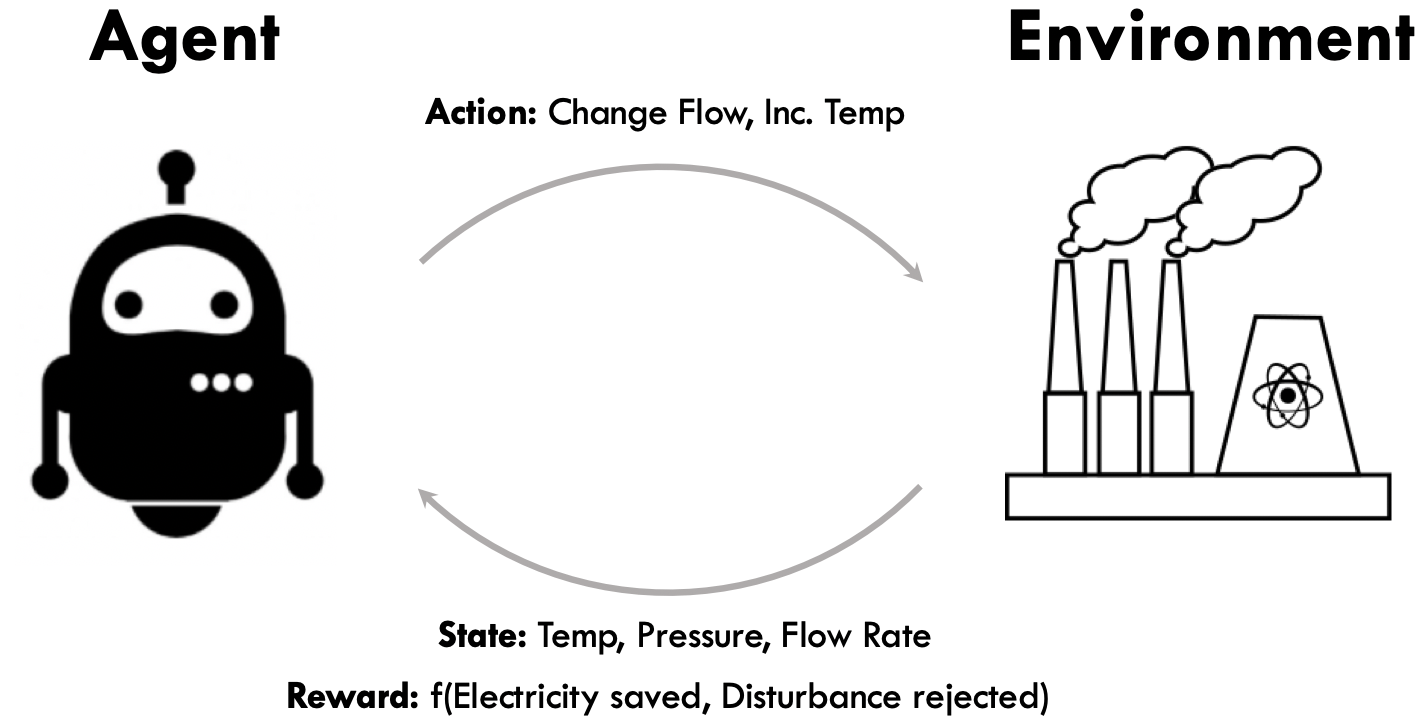
\includegraphics[scale=0.5]{images/ch1/RL.png}
    \caption{Basic setup of reinforcement learning where an agent interacts with the system.}
    \label{fig: simple_rl}
\end{figure}

The three main branches of reinforcement learning solutions are shown in Figure \ref{fig:RL_methods}. Starting from the left, dynamic programming (DP) methods can identify the exact value functions, but require a \textit{perfect system model} and is extremely computationally expensive, even for trivial tasks.  Comparatively, both Monte Carlo (MC) and temporal difference (TD) methods are approximate DP methods.  As such, they are less computationally demanding.  Additionally, MC and TD methods do not assume the presence of a system model and identifies the value functions through interactions with the environment. MC methods find the value functions through averaging the returns generated over many sampled trajectories of states, actions, and rewards.  One drawback is the significant variance in the sampled trajectories. Consequently, this may lead to poor reproducability in highly noisy systems. TD methods combine the best characteristics of DP and MC methods into one unifying approach. Like MC methods, TD learn from sampled data.  Like DP methods, TD performs update steps after each step. However, TD methods typically exhibit large bias (especially during initial learning episodes) due to estimating values through previously estimated values (known as bootstrapping). The general details of each method will be shown throughout this section.  For a comprehensive introduction to each algorithm, see \cite{sutton}.

\begin{figure}[H]
    \centering
    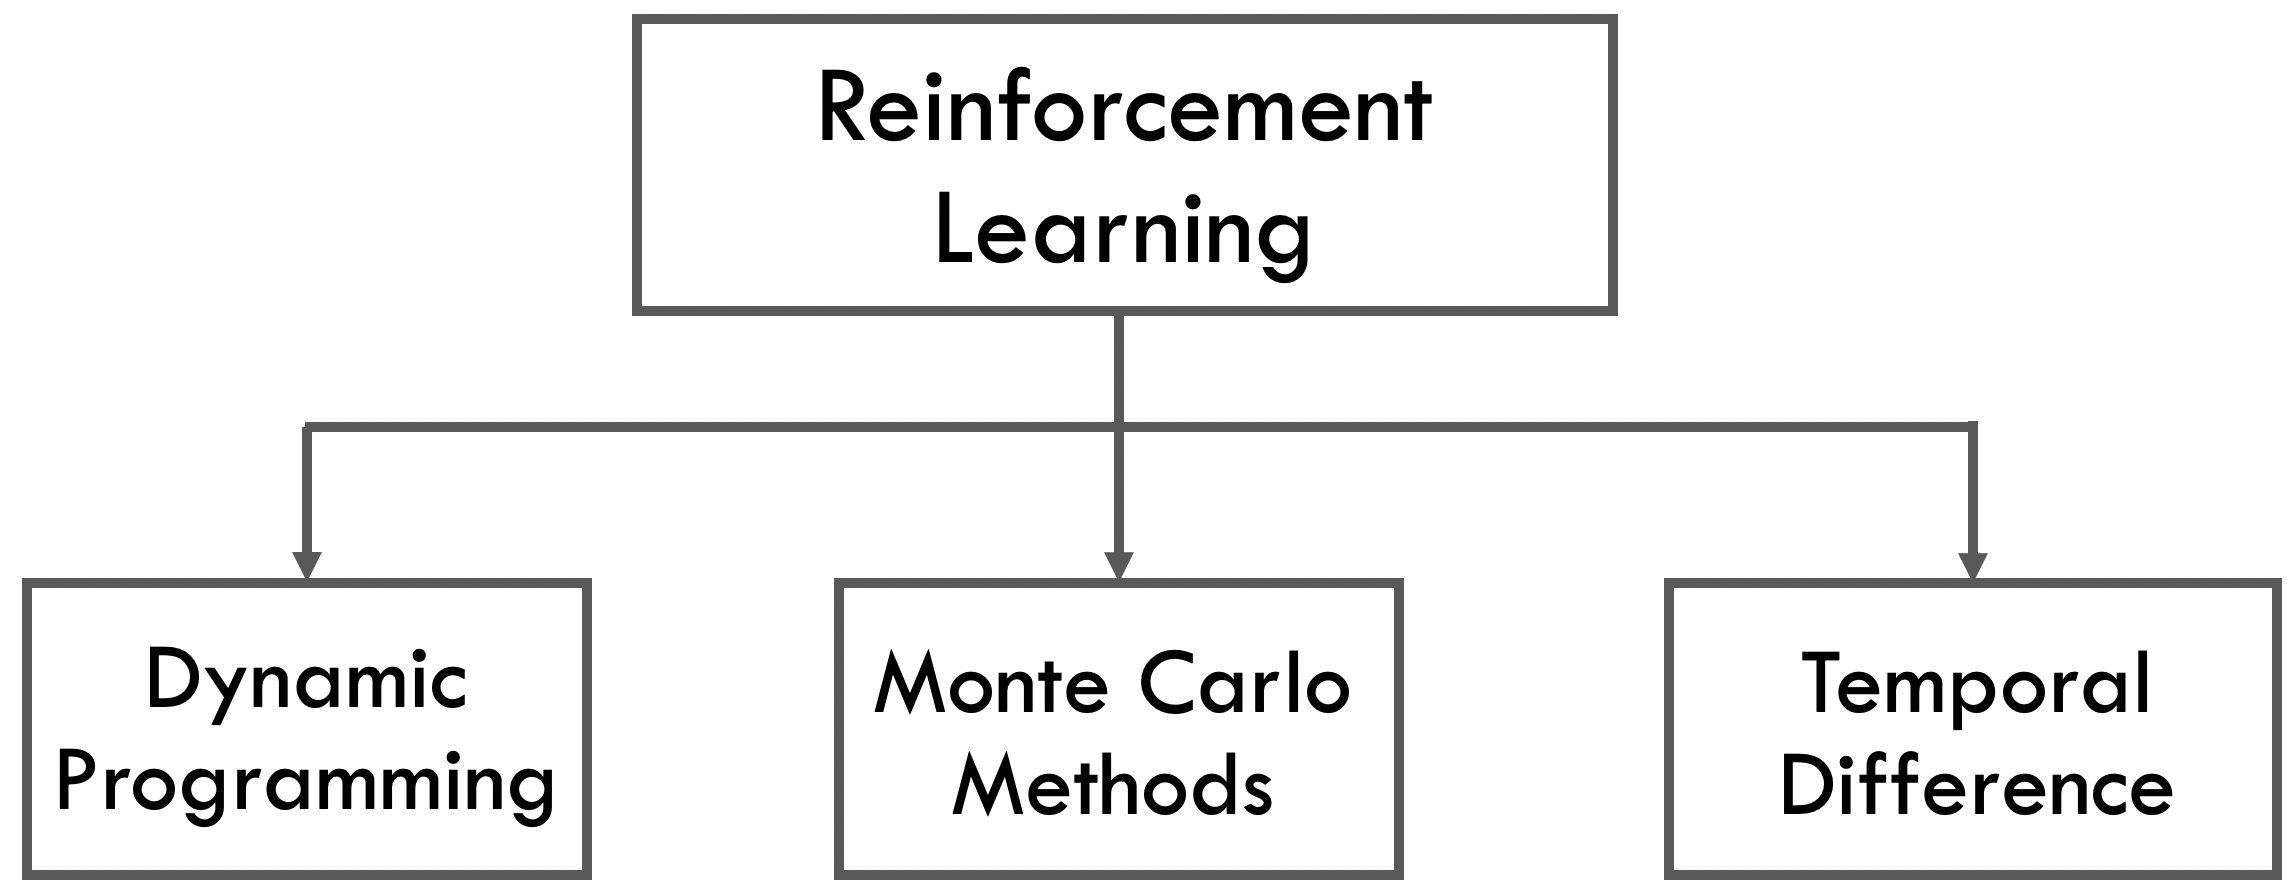
\includegraphics[width=0.6\textwidth]{images/ch1/RL_methods.jpeg}
    \caption{The sub-components of machine learning.}
    \label{fig:RL_methods}
\end{figure}   


\subsection{Dynamic Programming Methods}
Dynamic programming algorithms identify the exact value functions through an iterative procedure using the system dynamics function. In real life applications, DP algorithms are rarely used due to their unreasonable computational cost for even trivial problems. Problems are solved using either policy iteration and value iteration in DP.  

As an overview, policy iteration searches for the optimal policy by iterating through infinitely many policies, $\pi \in \Pi$, keeping only the policy with the highest cumulative returns.  The optimal policy is found when the cumulative returns of $\pi$ can no longer be improved (convergence).  Policy iteration includes two steps: policy evaluation and policy improvement. \textbf{Policy evaluation} predicts the value functions for policy $\pi$ through an iterative approach. Value functions for each state are initialized as 0, and are updated using:
\begin{equation}
    v_{k+1, \pi}(x) = \mathbb{E}_{\pi}[R_{t+1} + \gamma v_{k, \pi} (x_{k+1})]
\end{equation}
$$ v_0(x) = 0, \; \forall x \in \mathcal{X}$$
where $k$ is the $k^{th}$ update step.  Here, $v_{k+1, \pi}$ is the predicted value function for following policy $\pi$ after $k+1$ update steps.  As $k \rightarrow \infty$, $v_{k}(x) \rightarrow v_{\pi}(x)$ for all $x \in \mathcal{X}$ (i.e., the true value functions for $\pi$). However, there may exist a $\pi'$ where $v_{\pi'}(x) \geq v_{\pi}$, deeming $\pi$ sub-optimal. The goal of \textbf{policy improvement} is to identify situations where $v_{\pi'}(x) \geq v_{\pi}$ for any state.  Once identified, $\pi$ will violate the principle of optimality, hence disqualifying it from being optimal and $\pi'$ will be deemed the "new" optimal policy. This procedure will continue iteratively and infinitely until a policy where $v_{\pi^*}(x) \geq v_{\pi \neq \pi^*}(x)$ for all $x \in \mathcal{X}$ is found. 

\subsection{Monte Carlo Methods}
\subsection{Temporal-Difference Methods}

\subsection{Summary of the different solution approaches}
The main features of DP, MC and TD methods are summarized in Table \ref{tab:dc_mc_td}. Overall, DP requires a dynamics function of the system to compute the value functions while both MC and TD methods can learn directly from interactions with the system. Both DP and TD methods use bootstrapping to estimate value functions, that is, they estimate the current value function based on previously estimated values. Bootstrapping is data efficient, but introduces large bias to the estimated values, especially in the early episodes.  Conversely, MC methods estimate the value functions of each state independently through sampling many system trajectories.  However, this method, instead, introduces high variance. For extremely noisy systems, the reproducability of the results may be difficult. Comparing the computational cost, DP methods require much more compared to MC or TD since all value functions are simultaneously solved. In MC methods, only the value functions that were visited in the sampled trajectories are updated.  Additionally, updates are conducted at the end of each episode and not after each step. Similar to DP methods, TD methods update the value function immediately after an experience; however, only the value function corresponding to the last visited state is updated. In terms of exploration, DP methods do not explore the system model (both transition probabilities and expected reward) is explicitly provided. MC methods explore by being initiated in a random state after each episode termination. In TD methods, agents explore by occasionally performing a random action.

\begin{table}[H]
\caption{A comparison of DP, MC, and TD methods.}
\label{tab:dc_mc_td}
\centering
\begin{tabular}{c|c|c|c}
 & \textbf{Dynamic Programming}	& \textbf{Monte Carlo} & \textbf{Temporal Difference}\\
\hline
Requires model	     	& Yes			& No     &  No \\
Estimate bias           & High			& Low    &  High \\
Estimate variance	    & Low			& High   &  Low \\
Computational cost		& High			& Medium &  Low \\
$v(x)$ update      	& All states simultaneously   & After a trajectory  &  After an experience \\
Exploration             & Not needed, all states update   & Random initialization  &  Performing a random action \\
\end{tabular}
\end{table}

\subsection{Reinforcement Learning vs. Other "Learnings"}

Machine learning consists of the following four classes: i) Supervised learning, ii) Unsupervised learning, iii) Semi-supervised learning, iv) Reinforcement learning.  Supervised learning is fitting a model to map input data to output data.  The model is initially trained on a set of labeled training data provided by a subject matter expert.  Subsequently, unsupervised learning is used on unlabeled data sets.  The objective of unsupervised learning is to explore the data and identify hidden features. Semi-supervised learning combines the strengths of supervised and unsupervised learning, and is especially useful \cite{machine_learning}.  Often times, industrial data will be partially labelled due to the time and cost associated with data labelling.  For supervised and unsupervised learning, only the labeled and unlabeled data can be used, respectively.  However, all data can be used in semi-supervised learning which allows for maximized data efficiency and increased model performance. Finally, reinforcement learning is a goal-directed learning from interactions with the environment \cite{sutton}.

Reinforcement learning is a unique class of machine learning.  An ideal supervised learning model can only be as good as the subject matter expert providing the labels to the data set, which may not be 100\%.  For example, in a complex control task, the control law is usually highly non-linear. Control experts can try to provide control strategies for such systems, but optimality may not be guaranteed for highly non-linear systems. Also, supervised learning is used to generalize responses for occurrences not present in the data \cite{sutton}.  Reinforcement learning works by directly interacting with the environment \textit{without labels}. Through adequate exploration, reinforcement learning will identify peculiar features to optimally control such problems [citation required].  Reinforcement learning is \textit{similar} to unsupervised learning in terms of identifying hidden structures within the environment.  However, reinforcement learning tries to maximize an internal scalar "reward" signal, rather than purely data mining.

Evolutionary methods, a family of optimization algorithms such as genetic algorithm, are most similar to reinforcement learning.  For a control problem, such methods can apply multiple static policies for different operating regimes \cite{sutton}.  Policy search is conducted by first initiating $k$ random input trajectories of length $N$, generating input matrix $\mathbb{U}_{[k, N]} \in \pi$.  Subsequently, the loss, $J_U$, of each $U$ is calculated based on the objective function.  Input trajectories with the lowest loss move onto the next generation and generates new pseudo-random input trajectories.  This process is repeated until optimal policy, $\pi^*$ is found for each operating regime \cite{ga_for_control}.

Evolutionary methods work well when the policy space is sufficiently small, easy to find, or a lot of time is available for optimization.  The biggest advantage of such methods compared to reinforcement learning is that the whole state does not need to be known.  However, such methods does not capture the reinforcement learning fundamentals of mapping $X \rightarrow U$.  Unlike evolutionary methods, reinforcement learning keeps memory of each individual interaction making it a more data efficient approach \cite{sutton}.

%%%%%%%%%%%%%%%%%%%%%%%%%%%%% End Section Intro to RL %%%%%%%%%%%%%%%%%%%%%%%%%%%%%%%%%%%%%%%


%%%%%%%%%%%%%%%%%%%%%%%%%%%%% Begin Section Tabular RL %%%%%%%%%%%%%%%%%%%%%%%%%%%%%%%%%%%%%%

\section{Tabular Q-learning}

A detailed numerical example is provided in Chapter 4 where a tabular $Q$-learning algorithm was applied onto a physical pump system.

\subsection{Introduction to Q-learning}
\subsubsection{Adaptation to Non-Stationary Problems}
- explanation
\subsubsection{Exploration in Tabular Q-learning}
- epsilon greedy, ucb
\subsubsection{Reward Functions}
- mse, with action, etc



%%%%%%%%%%%%%%%%%%%%%%%%%%%%% End Section Tabular RL %%%%%%%%%%%%%%%%%%%%%%%%%%%%%%%%%%%%%%%

%%%%%%%%%%%%%%%%%%%%%%% Begin Section Function Approximation %%%%%%%%%%%%%%%%%%%%%%%%%%%%%%%

\section{Function Approximation}
\subsection{Introduction to Function Approximations}
- capture the data of large data set and condense it down into something smaller.
\subsection{Neural Network Basics}
\subsubsection{Neural Network Initialization}
\subsubsection{Gradient Descent Updating}
\subsubsection{Mini-batch Gradient Descent}
\subsubsection{Batch Normalization}
\subsubsection{Regularization}

%%%%%%%%%%%%%%%%%%%%%%%%% End Section Function Approximation %%%%%%%%%%%%%%%%%%%%%%%%%%%%%%%


%%%%%%%%%%%%%%%%%%%%%%%%%%%%%%%%% Begin Section DDPG %%%%%%%%%%%%%%%%%%%%%%%%%%%%%%%%%%%%%%%

\section{Deep Deterministic Policy Gradient}
\subsection{Actor-Critic Intuition}
\subsection{Actor - Deterministic Policy Gradient}
\subsection{Critic - Deep Q-learning}

\newpage

\subsection{Exploration in DDPG}
Traditionally, exploration in continuous action spaces are difficult because classical approaches, such as $\epsilon$-greedy, work only in a discrete action space.  DDPG explores through corrupting the action with exploratory noise \cite{ddpg}.  Throughout RL literature, many researchers conduct exploration using white noise. The noise corrupted action is given by:
\begin{equation}
    u'(x_t) = u(x_t|w_t) + \mathcal{N}
    \label{eq:01noise_corrupt}
\end{equation}
where $u'(x_t)$ is the action corrupted by some noise, $\mathcal{N}$.

\subsubsection{Exploration using White Noise}
In Equation \ref{eq:01noise_corrupt}, $\mathcal{N}$ can bewhite noise drawn from $\mathcal{N}(0, \sigma^2)$; however, white noise is de-correlated and is ineffective for "deep" exploration (i.e., traversing far from the current state) due to the zero averaging effect \cite{white_noise}. Intuitively, white noise simply introduces oscillation into the process and does not create displacement in any particular direction. Therefore, it is more effective to corrupt the action using a temporally correlated process such as the Uhlenbeck-Ornstein (UO) process.

\subsubsection{Ornstein-Uhlenbeck Exploratory Noise}

The UO process is given as \cite{ornstein}:
\begin{equation}
    dx_t = \theta x_t dt + \sigma dW_t,
\end{equation}
where $\theta > 0$, $\sigma > 0$, and $W_t$ denotes the Wiener process. Mathematically, the Wiener process is a special case of a continuous time stochastic process. Detailed information regarding the Wiener process and its properties can be found in \cite{wiener}. The UO process is ideal for exploratory noise in RL because of its time correlated feature.

Intuitively, actions $u_t$ from the RL agent can be understood as exerting an external force upon physical bodies and is given by Newton as \cite{physics}:
\begin{equation}
    u = m \ddot{x}
\end{equation}
where $m$ denotes mass and $\ddot{x}$ represents acceleration.  To obtain displacement, the force must be integrated twice:
\begin{equation}
    x = \frac{1}{m}\int \int u
\end{equation}
Interestingly, the integration operator acts as a low-pass filter and removes all high frequency noise contained in $u$ \ref{process_control_ref13}. Assuming that the noise is temporally correlated, such as the UO process, the displacement will typically be smooth and stay in the same direction for long durations. For example, Figure \ref{fig:01OU} 

\begin{figure}[H]
    \centering
    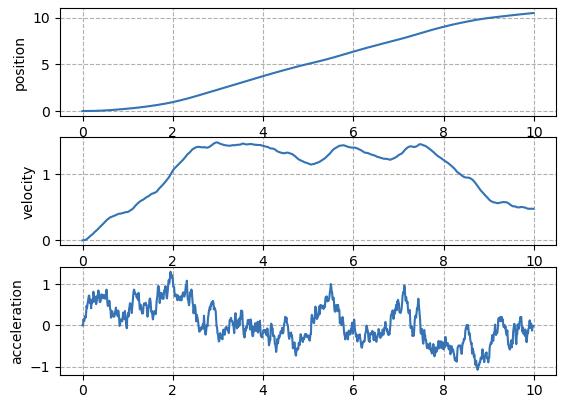
\includegraphics[width=0.56\textwidth]{images/ch1/01OU.jpeg}
    \caption{Change in position as a function of different}
    \label{fig:01OU}
\end{figure}   





\subsection{Stabilization of Training}
\cite{dqn1, dqn2, ddpg, ornstein, wiener}
\subsubsection{Experience Replay}
\subsubsection{Target Network}
\subsubsection{Adaptive Batch Gradient Descent}
\subsubsection{Reward Clipping}
\subsection{Input and State Constraints}
\subsection{Training Algorithm}

%%%%%%%%%%%%%%%%%%%%%%%%%%%%%%%%%% End Section DDPG %%%%%%%%%%%%%%%%%%%%%%%%%%%%%%%%%%%%%%%%
